
\item A ball of radius \( R = 10.0\ cm \) rolls without slipping down an inclined plane so that its centre moves with constant acceleration
    \begin{center}
        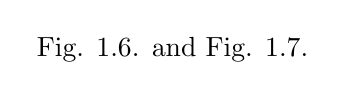
\begin{tikzpicture}
            \node at (0, 0) {Fig. 1.6. and Fig. 1.7.};
            % Diagrams should be drawn here according to the actual diagrams in the image provided
        \end{tikzpicture}
    \end{center}
    \begin{enumerate}
        \item \( w = 2.50\ cm/s^2; \quad t = 2.00\ s \) after the beginning of motion its position corresponds to that shown in Fig. 1.7. Find: the velocities of the points \( A, B, \) and \( O; \)
        \item the accelerations of these points.
    \end{enumerate}
\begin{solution}
    \begin{center}
        \begin{tikzpicture}
            \pic at (0, 0) {frame=3cm};
        \end{tikzpicture}
    \end{center}
    
    \begin{align*}
        \intertext{As the ball rolls without slipping on the rigid surface along a line so, contact point O has zero velocity, which is possible when the ball rotates in clockwise sense if its centre moves towards right and such that \(v_C = \omega R\) and \(w_C = \beta R\). As motion starts at \(t = 0\) with constant acceleration \(w\) so at time \(t\), the velocity of mass centre \(C\) becomes \(v_C = wt\) and \(\omega = \dfrac{v_C}{R} = \dfrac{wt}{R}\).}
        \intertext{(a) The contact point O becomes instantaneous centre of rotation, thus, the velocity of any arbitrary point P (say) of the ball can be obtained by the relation}
        \vec{v}_P &= \omega \times \rho_{PO} \tag{1}
        \intertext{Using Eq. (1), the pictorial diagram to find the velocities of the points A and B of the ball is shown below}
        \intertext{Hence,}
        v_A &= 2v_C = 2wt = 10 \text{ cm/s}\\
        \text{and} \quad v_B &= \sqrt{2} \; v_C = \sqrt{2} \; wt = 7.1 \text{ cm/s}
        \intertext{(b) One can write for the any arbitrary point \(P\)}
        \vec{w}_P &= \vec{w}_C + \vec{w}_{PC} = \vec{w}_C + \omega^2 \; (-\rho_{PC}) + (\beta \times \rho_{PC}) \tag{2}
        \intertext{Taking into account Eq. (2), one can easily get the acceleration of the points O, A and B on using the pictorial diagram.}
        \intertext{So,}
        w_0 &= \dfrac{w t^2}{R} = 2.5 \text{ cm/s}^2\\
        w_A &= \sqrt{4w^2 + \dfrac{w^4 t^4}{R^2}} = 2w \sqrt{1 + \left(\dfrac{w t^2}{2R} \right)^2} = 5.6 \text{ cm/s}^2\\
        \text{and} \quad w_B &= \sqrt{\left(w - \dfrac{w t^2 t^2}{R} \right)^2 + w^2} = 2.5 \text{ cm/s}^2
    \end{align*}
\end{solution}